\documentclass[adobefonts, nocap]{ctexart}
\usepackage{amsmath}
\usepackage{amsfonts}
\usepackage{listings}
\usepackage{xcolor}
\usepackage{graphicx}
\usepackage{siunitx}
\usepackage{hyperref}
\hypersetup{
  colorlinks = true,
  linkcolor = blue,
  unicode = true
}
\lstset{
  language = C,
  basicstyle = \small\ttfamily,
  keywordstyle = \small\ttfamily\color{red},
  stringstyle = \color{gray},
  numbers = left,
  numberstyle = \tiny,
  numbersep = 5pt,
  frame = leftline,
  showstringspaces = false
}
\begin{document}
  \title{分支预测读书报告}
  \author{李雨田\hspace{1em}2010012193\hspace{1em}计14}
  \maketitle
  \tableofcontents
  \section{概述}
    为提高流水线处理机和超标量处理机的性能,人们提出了多种方法来预测指令流执行的路径.分支预测用来解决控制冲突带来的取指令的瓶颈,
    以达到指令级并行.一般程序平均20\%是分支指令,没有分支预测的话,每次执行分支指令处理机都要暂停.如果
    分支预测准确率足够高,处理机的性能将得到极大提升.
  \section{分支指令属性}
    \subsection{基本属性}
      分支指令总的来说有三个基本属性:分支指令的类型,分支指令发生的频率和分支指令的成功率.分支指令的类型可以分为条件分支指令和无条件分支指令,由于分支指令目标地址的不同,无条件分支又可以进一步分为立即分支指令,间接分支指令和返回分支指令.立即分支指令就是分支的地址就在分支指令中.一般都是直接跳转,比如跳转(jump)这类指令.间接分支就是分支的目标地址不在分支指令中,而是从其他寄存器中取得.返回型分支的分支目标地址是从链接寄存器(Link register)或者堆栈中得到,一般是程序返回使用.

      统计分析SEPC程序结果表明,分支指令中$72\%$是条件分支, $17\%$是无条件立即跳转指令, $10\%$是返回指令, $1\%$是间接分支指令.其中立即分支跳转可以采用BTB (Branch Target Buffer,分支预测缓冲区)这种方式精确预测,返回型跳转可以采用返回地址栈(RAS1)精确预测,间接分支跳转的预测一直没什么好的办法.所以分支预测大量的工作是进行条件分支预测.

      由SPEC程序条件分支预测执行的频率分布可以看到,大部分条件分支在程序运行过程中,仅仅执行几次,平均来说所有分支指令的$53\%$仅仅执行$99$次或者更少,只有$11\%$的分支执行了超过$10000$次或者更多.

      考虑不同分支指令执行在整个程序分支的权重,上面所说的执行$99$次或者更少的分支指令有$53\%$,执行$99$次或者更少的分支指令占SPEC程序的$53\%$,但是这$53\%$的指令在SPEC程序分支执行比重中只占$0.2\%$,在柱状图上都显示不出来.而占$11\%$的分支指令占据了所有分支执行的$87\%$,也就是$10\%$的指令占据了程序$90\%$的运行时间.

      分支成功率是分支指令成功跳转除以整个程序运行的分支总数.从统计可以看出来大概$28\%$的指令总是跳转或者总不跳转,另外有$32\%$的指令,跳转的几率总少于$5\%$或者多于$95\%$总跳转,也就是说$60\%$的分支指令具有强烈的一个跳转方向,所以可以推出,具有挑战性的工作是预测其余$40\%$的分支跳转.
    \subsection{程序的分支属性}
      我们所运行的程序中有大量的分支指令,这些指令组合起来就表现为程序的分支行为,不同应用程序的分支行为非常复杂.国际上对分支预测的研究一般都主要针对SPEC CPU的程序,因为SPEC程序是专业测试机构精心挑选出来的,在各个行业有代表性应用的一组程序,一般国际上都是通过对比SPEC的分数来说明处理器性能.对SPEC测试程序的分析表明$5$到$7$条指令里面就有$1$条分支指令,而处理器一般都是一次取$4$到$6$条指令,也就是说几乎每次都可能取到一条分支指令,这进一步说明了对分支指令研究的重要性,甚至有文章认为分支预测将来可能是处理器性能提高的瓶颈.

      总体而言程序分支行为有以下特点,循环结构在现在程序中大量存在.大量的研究表明,循环结构的分支指令行为在程序中是最为常见,重复出现的一种分支模式.一般我们可以用一个字符串来记录程序循环模式,比如一个循环$10$次的程序可以用$1110100110$来表示,其中$0$代表不跳转,$1$代表跳转.前文已对分支指令的属性作了说明和分类,而多条分支指令组合成程序的分支行为,可以根据循环的模式来进行分支预测,这些模式在SPEC程序几十亿指令的执行过程中会重复出现.

      程序分支属性存在系统性,或者联想性.这种形式不重复出现,但是大量存在,例如SPEC的parse程序分析一个单词"chines",它自然会预测到下一个字母是e,研究中表明$30\%$的分支有这样的系统推测行为.但是由于程序的行为非常复杂,目前这方面研究还没什么太大进展.研究表明如果一段程序中,程序分支之间有相关性.相关性一般多出现在程序的if-else分支.两条同样类型的分支指令有相反的分支结果,一般这两条分支指令是相关的.这就告诉我们如果预测成功其中一条分支指令,就可以知道另外一条分支指令的预测结果.以前的研究表明$60\%$的分支指令具有相关性,这也成为后面分支预测的主要基础.
  \section{静态分支预测}
    要了解动态分支预测,要首先了解静态分支预测.静态分支预测使用程序运行前的到的信息,预测分支.

    最简单的分支预测机制是MIPS-X上的总是转移和Motorola MC88000上的总是不转移.另一种静态分支预测的方法
    是使用训练输入运行一遍程序,收集分支转移的信息作为分支转移的预测.
  \section{动态分支预测}
    动态分支预测使用运行时收集的信息来预测分支转移.一般包括一级分支预测,二级分支预测,和混合
    分支预测.
    \subsection{一级分支预测}
      最简单的一级分支预测使用直接映射的形式.使用分支指令地址的低$k$位作为索引,映射到一个饱和计数器
      上.每次分支转移,计数器加一,否则减一.加到最大值就不再增加,减到最小值也不在减少了.当饱和计数器
      的值小于最大值的一半的时候就预测分支不转移,否则预测分支转移.这就是
      饱和计数器的工作原理.

      就像处理机缓存一样,除了直接映射,还有组映射和全相关映射等方法讲分支指令地址映射到相应的饱和计数器.
      或者使用一定的哈希函数做映射.

      饱和计数器可以是任意$n$比特,不过常用$2$比特的饱和计数器,在性能和存储空间之间达到一个较好的平衡.

      \begin{center}
        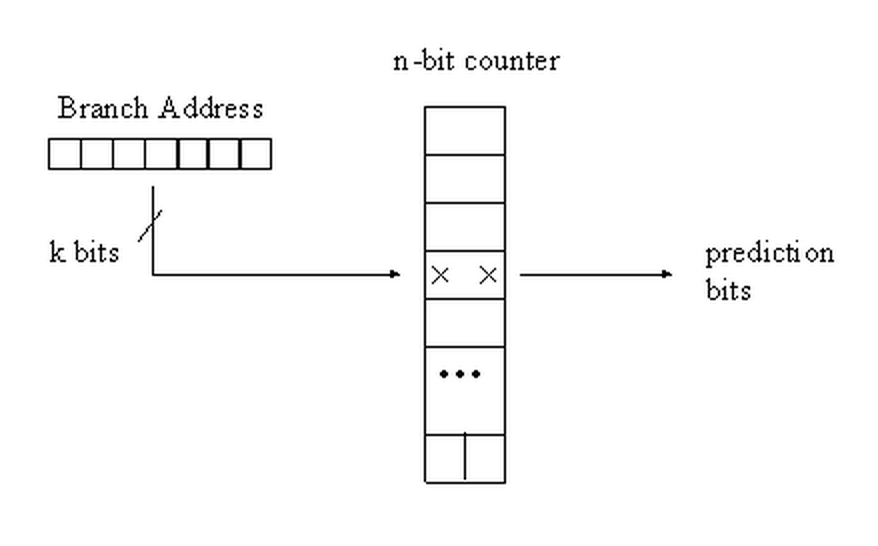
\includegraphics[width=10cm]{1.png}
      \end{center}
    \subsection{二级分支预测}
      二级分支预测由Yeh和Patt发明,使用多个信息来源来定位相应的饱和计数器.一般会有一个全局
      分支历史,对于分支转移,左移进$1$,否则左移进$0$.还有一个局部历史表,每个寄存器对应于
      一个具体的分支指令,同样,如果分支转移,左移进$1$,否则左移进$0$.但是由于局部历史表
      大小的限制,很可能多个分支指令对应于一个表项,就有了重名失真的问题.所以一般情况下局部历史表
      越大越好.

      这样就能构造一个二维的表,根据全局分支历史和分支指令地址就可以定位到相应的饱和计数器.
      饱和计数器的操作同上.

      \begin{center}
        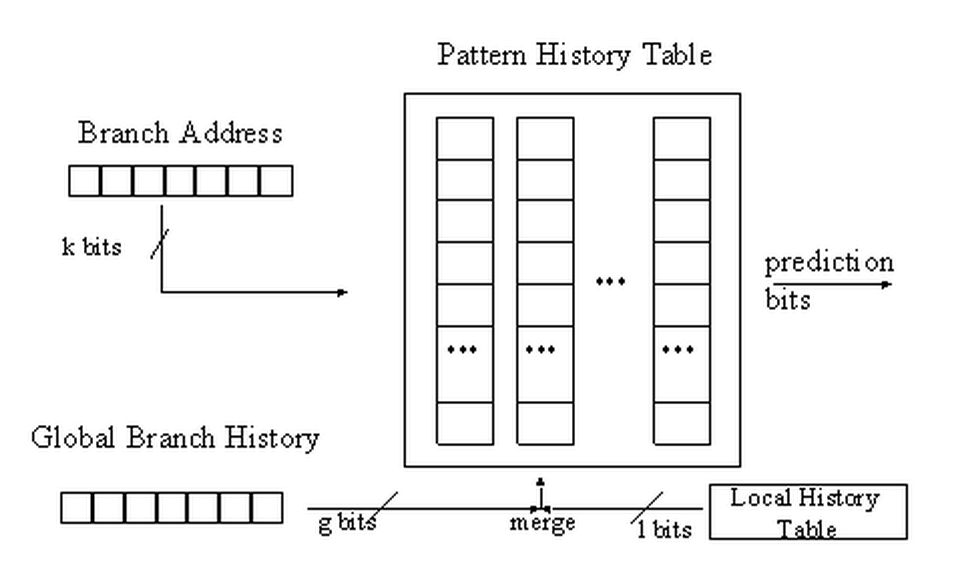
\includegraphics[width=10cm]{2.png}
      \end{center}

      而全局分支历史和分支指令地址的合并一般有两种方法.

      \begin{enumerate}
        \item 连接.可以取分支指令地址的几位和全局分支历史的几位合并.
        \item 异或.将两个地址异或起来.
      \end{enumerate}

      \begin{center}
        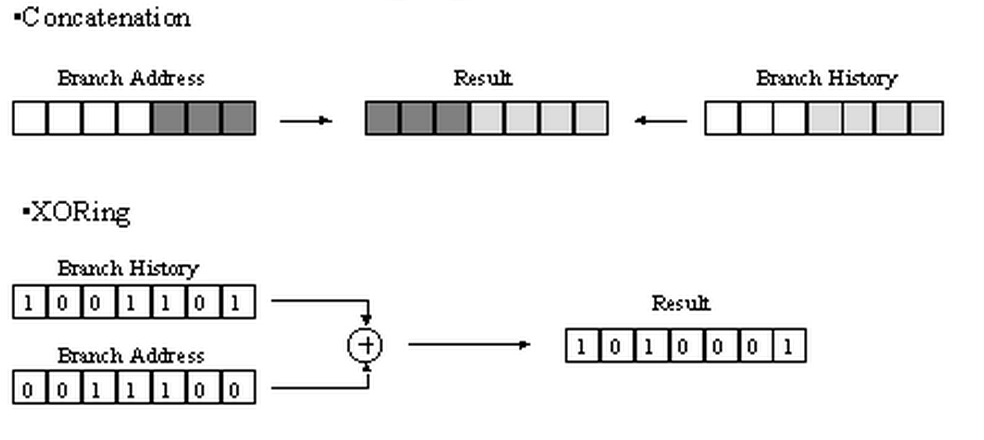
\includegraphics[width=10cm]{3.png}
      \end{center}

      实验显示,一般情况下异或的效果更好.说明异或更能避免合并带来的重名失真的问题.

      可以认为二级分支预测比一级分支预测的效果更好,但是带来的问题就是需要更多的存储空间,
      实现起来更加困难和昂贵.而且预热的时间更长,需要更长的时间来初次填充饱和计数器.在预热的时候
      准确率是没有保障的.而且如果操作系统上下文切换频繁,则预热的问题将更加显著.
    \subsection{混合分支预测}
      混合分支预测由McFarling最初提出.综合两个不同的预测机制,由两个预测机制独立给出结果.
      并且再维护一个饱和计数器,来决定相信哪个预测机制的结果.饱和计数器也会更新,偏向于经常给出
      正确结果的预测机制.

      这样的好处就是,可以结合一个准确率高但是预热慢的预测机制和一个预热快但是准确率不是很高的
      预测机制.在程序运行一开始,偏好于预热快的机制.当准确率高的机制预热完毕后,则可以转换到
      准确率高的机制.有效结合了不同预测机制的优点.

      混合分支预测可以推广大于两个预测机制,由Patt提出.具体每个组成成分有很多种选择,例如

      \begin{enumerate}
        \item 2bC
        \item GAs
        \item PSg
        \item gshare
        \item pshare
        \item loop
      \end{enumerate}
  \section{分支预测实现}
    \subsection{Decode History Table}
      直接使用分支指令地址的低$k$位索引.在硬件的实现上是最简单的.

      \begin{center}
        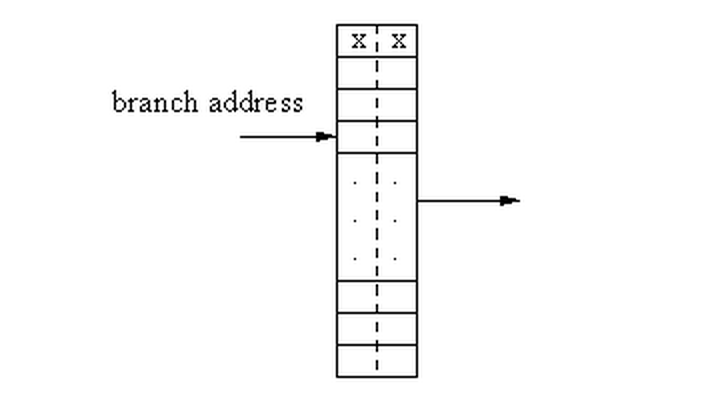
\includegraphics[width=10cm]{4.png}
      \end{center}
    \subsection{Branch History Table}
      和Decode History Table类似.但是在索引到相应的项后,会和完整的分支指令地址进行对比.
      如果不对则预测不转移.这样的实现完全消除了重名失真的问题.但是对于直接映射的分支预测,
      这种方法并没有带来性能上的提升.

      \begin{center}
        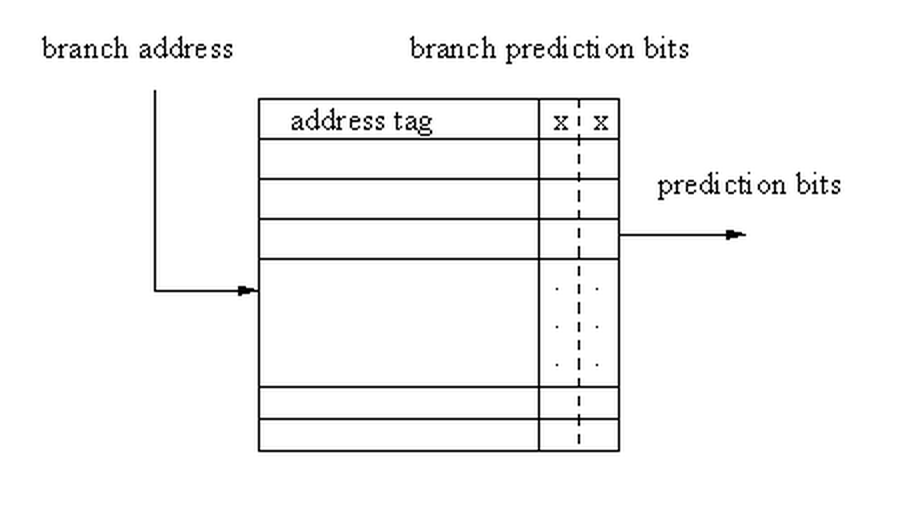
\includegraphics[width=10cm]{5.png}
      \end{center}
    \subsection{Combination of DHT BHT}
      结合以上两种实现,这种实现一般情况下使DHT比BHT大很多,来达到硬件上的平衡.这是一种混合
      分支预测的实现.

      \begin{center}
        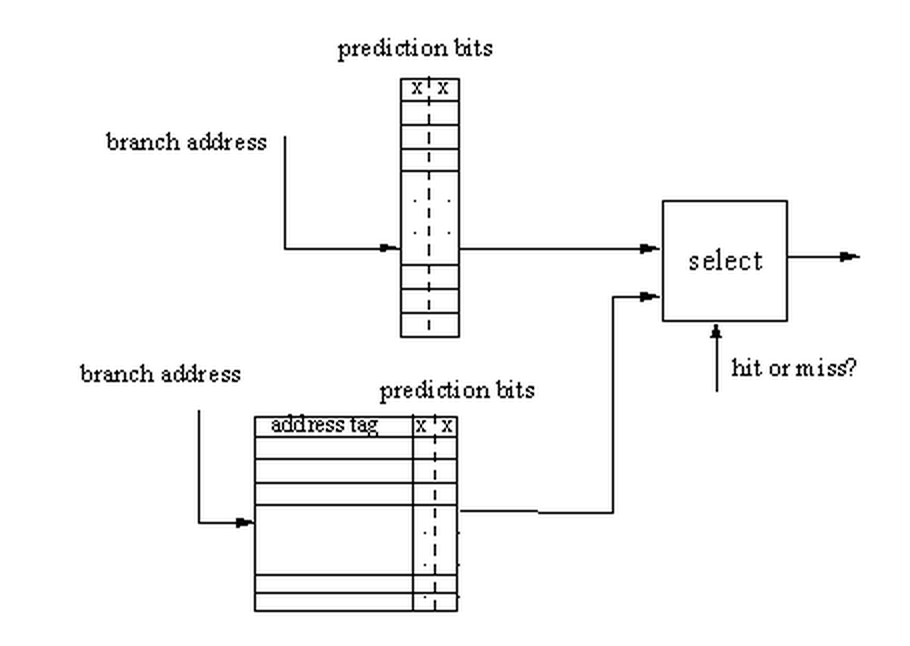
\includegraphics[width=10cm]{6.png}
      \end{center}
    \subsection{Correlation Based Prediction}
      Correlation Based Prediction和之前的方法不同的是,预测不仅依赖本分支之前的行为,
      还依赖之前执行的分支的结果.指令流里之前分支执行的结果存在一个全局的寄存器中,如果分支转移,
      则左移进$1$,否则左移进$0$.预测用表是二维的,用分支指令地址选取行,用全局寄存器中的值选取列.

      之所以这样设计,是因为一个分支的行为不仅和它自己之前的行为有关,还和其他分支的执行情况有关.
      将这两者结合起来,可以利用其相关性达到更好的结果.这种方法在硬件上更加复杂.

      \begin{center}
        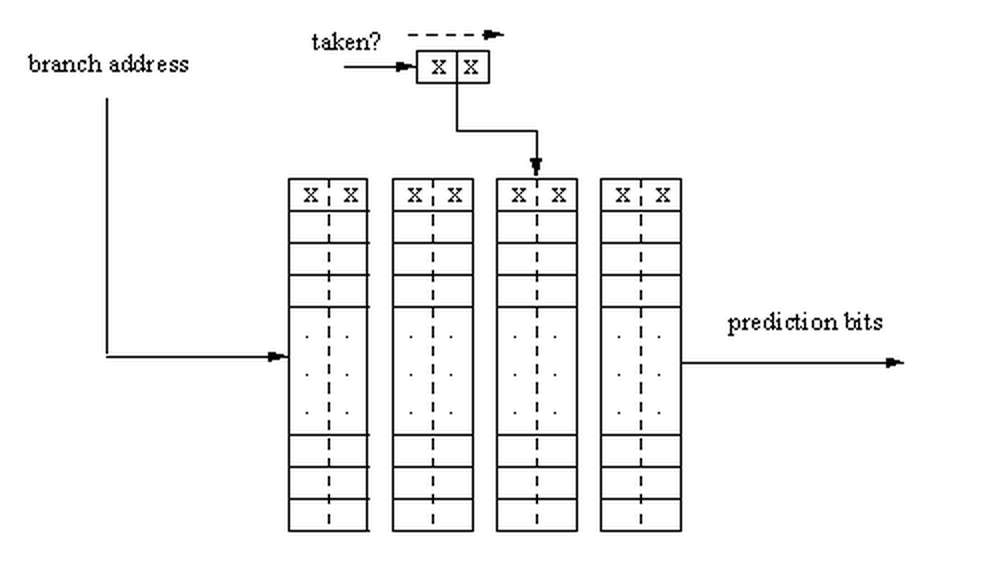
\includegraphics[width=10cm]{7.png}
      \end{center}
    \subsection{Two Level Adaptive Prediction}
      Two Level Adaptive Prediction最初由Yeh提出.像之前所述的方法,也使用了之前分支的结果.
      但是这个信息不是全局保存的,而是保存在局部的寄存器中.对于每一个分支指令地址,都有一个
      关联的相关性寄存器.根据这个信息,再检索Global Pattern Table中的饱和计数器. Two Level
      Adaptive Prediction比Correlation Based Prediction好在要求的硬件成本更低.

      \begin{center}
        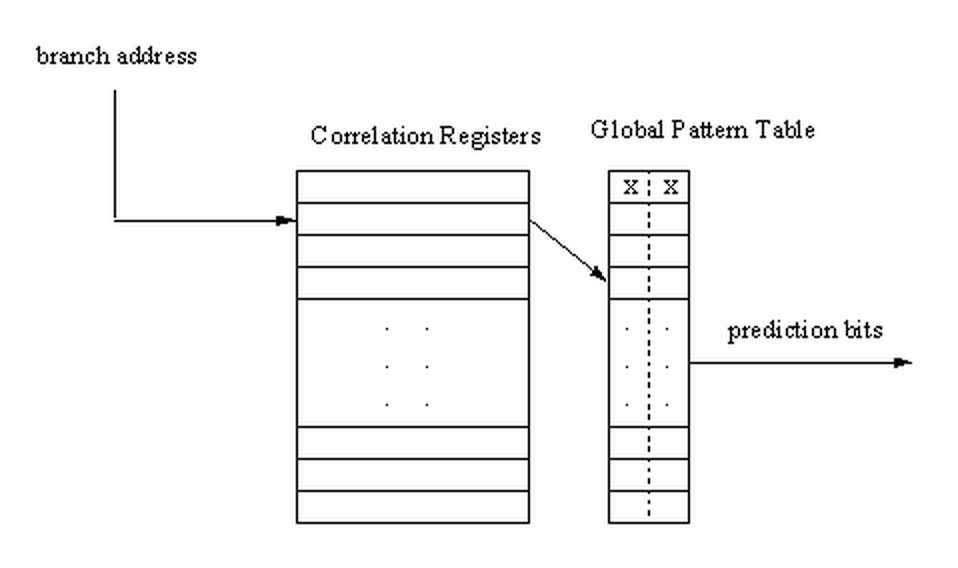
\includegraphics[width=10cm]{8.png}
      \end{center}
    \subsection{Skewed Branch Predictor}
      Skewed Branch Predictor也使用了全局历史,就像Correlation Based Prediction一样.
      它使用全局历史和分支指令地址,和不同的哈希函数,从三个不同的独立的预测机制里得到三个预测结果.
      最后使用多数派的结果作为预测结果.

      更新的时候,三个预测机制都要相应更新.这个方法由Michard提出,能够消除大部分的重名失真.

      \begin{center}
        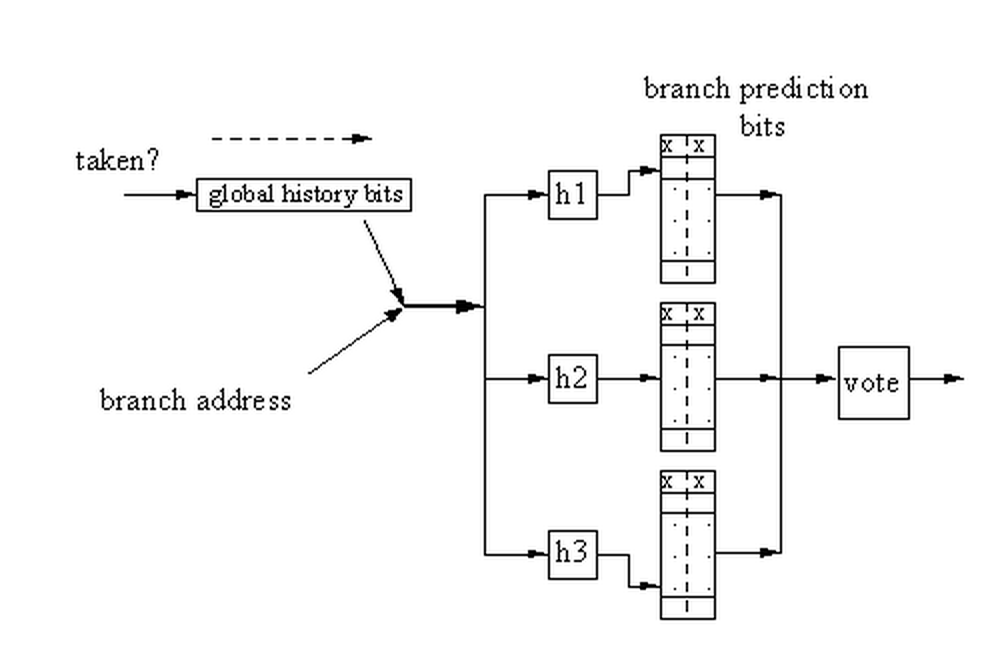
\includegraphics[width=10cm]{9.png}
      \end{center}
    \subsection{Gshare}
      Gshare和Branch History Table类似,但是它会先将分支指令地址和全局历史异或在一起.具体
      实现可以使用有完整分支指令地址,如果地址不吻合则预测不转移.如果吻合,则使用对应的预测结果.
      在没有分支指令地址的实现中,则直接使用预测结果.

      虽然看起来使用完整分支指令地址会占用更多的硬件空间,按道理会得到更好的效果.实验结果却
      表明不使用完整分支指令地址的效果更好.并且在硬件空间上,和Bimodal Predictor相同.

      \begin{center}
        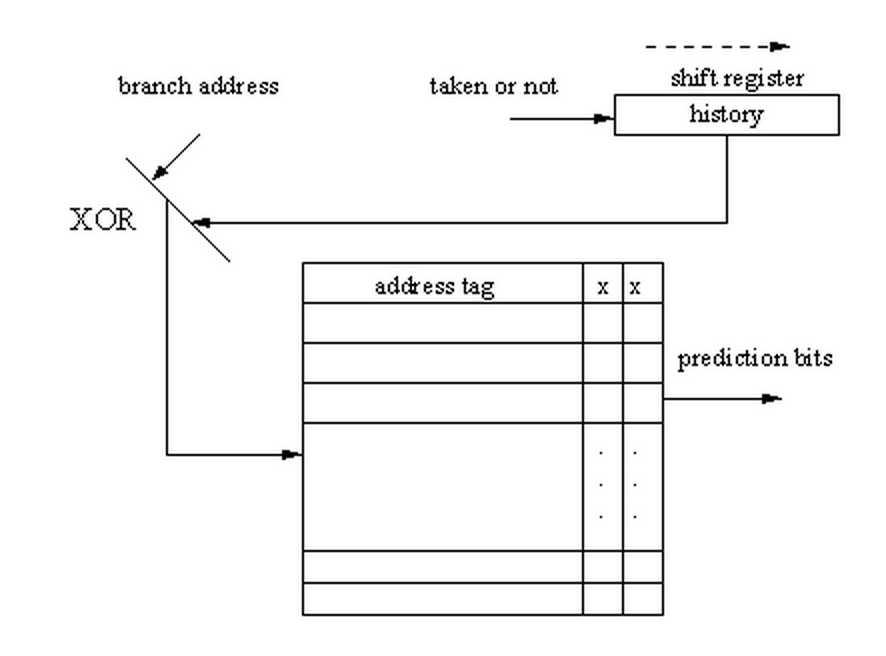
\includegraphics[width=10cm]{10.png}
      \end{center}
    \subsection{Branch Target Address Buffer}
      以上都只考虑了分支预测的正确性,但是即使预测正确,还是要计算分支目的指令.为了解决这个问题,
      可以预先计算分支目的地址,将其存在Branch Target Address Buffer里面.实际运行时一旦
      预测分支转移,则可以里面得到目的地址,加快运行速度.
  \section{总结}
    综上所述,分支预测的发展一直伴随着高性能处理器的发展,分支预测器对处理器性能提高起着重要作用,一直都是处理器设计的重中之重.
    历史上出现了多种不同的分支预测的方法,它们也各有优点和缺点.但是它们都在一定时期占据过市场的主流.
    可见并不是性能最优的方法就是最好的,在具体的工程实践中,还要考虑到设计和成本等多种因素.随着时代的变迁,
    器件成本下降,越来越好的分支预测的方法得以普及,大大提升了处理机的性能.

    但是,分支预测器设计中如何平衡功耗是个大问题.目前神经网络分支预测器是学术界的研究热点,可以预见近期这方面研究将有可能取得大的进展.
  \section{参考文献}
    \begin{enumerate}
      \item Dynamic Branch Prediction\\(http://web.engr.oregonstate.edu/\~benl/Projects/branch\_pred/)
      \item Dynamic Branch Prediction\\(http://courses.cs.washington.edu/courses/csep548/06au/lectures/branchPred.pdf)
      \item Combining Branch Predictors\\(http://www.hpl.hp.com/techreports/Compaq-DEC/WRL-TN-36.pdf)
      \item Branch Target Buffer\\(http://web.cs.dal.ca/~mheywood/CSCI3121/Pipe/05-BTB.pdf)
      \item 处理器分支预测研究的历史和现状\\(http://www.chinadmd.com/file/3vsavvvtuxo3cppc3pexzxvc\_1.html)
    \end{enumerate}

\end{document}
